% Uncomment this to make slides with overlays:
% \documentclass[slides]{beamer}

% Uncomment these (but comment the above \documentclass line) to make handouts:
\documentclass[handout]{beamer}

% Uncomment these to have more than one slide per page
\usepackage{pgfpages}
\pgfpagesuselayout{2 on 1}[border shrink=5mm]
\pgfpageslogicalpageoptions{1}{border code=\pgfusepath{stroke}}
\pgfpageslogicalpageoptions{2}{border code=\pgfusepath{stroke}}

\usepackage[]{graphicx, color, hyperref}

\mode<presentation>
{
	%\usetheme[secheader]{Boadilla}
	%\usecolortheme[rgb={.835, .102,.169}]{structure}  
	\usetheme[width= 0cm]{Goettingen}
	%\setbeamercovered{transparent}
}
\setbeamertemplate{navigation symbols}{}
\setbeamertemplate{footline}[frame number]

\definecolor{blue2}{rgb}{0.278,0.278,0.729} 
\newcommand{\blue}[1]{\textcolor{blue2}{#1}}
\newcommand{\white}[1]{\textcolor{white}{#1}}
\newcommand{\red}[1]{\textcolor{red}{#1}}
\newcommand{\xbar}{\overline{x}}
\newcommand{\ybar}{\overline{y}}
\newcommand{\phat}{\widehat{p}}
\newcommand{\prob}{\mbox{Pr}}
\newcommand{\E}{\mathbb{E}}
\newcommand{\Var}{\mbox{Var}}
\newcommand{\cp}{\oplus}
\newcommand{\cm}{\circleddash}


\title{Lecture 23: Tests for Independence in Two-Way Tables}
\author{Chapter 6.4}
\date{}


\begin{document}
%------------------------------------------------------------------------------
\begin{frame}
\titlepage
\end{frame}
%------------------------------------------------------------------------------


%------------------------------------------------------------------------------
\begin{frame}
\frametitle{Quiz 9}

\blue{Question}:  While the results of the controlled experiment suggesting that women are at a disadvantage in science hiring may come as no surprise, what argument is made that this discrimination is not entirely due to overt misogyny?  Answer in one sentence.

\vspace{0.5cm}

\pause \blue{Answer}: Women rated women candidates lower as well, suggesting not so much explicit misogyny, but rather manifestation of subtler prejudices internalized from societal stereotypes.

\end{frame}
%------------------------------------------------------------------------------


%------------------------------------------------------------------------------
\begin{frame}
\frametitle{Quiz 9}

\blue{Question}:  Knowing nothing else about the problem (sample sizes, SE, etc), what can we conclude about the difference in means between men and women?

\vspace{0.5cm}

\pause\blue{Answer}: No, refer to HW8 Question 7.  We had two overlapping CIs, but the CI on the difference did not include 0.

\end{frame}
%------------------------------------------------------------------------------


%%------------------------------------------------------------------------------
%\begin{frame}
%\frametitle{Previously... Chi-Square Tests}
%
%Chi-square $\chi^2$ tests allow us compare \blue{observed} counts to \blue{expected} counts.
%
%\vspace{0.5cm}
%
%\pause We compute a $\chi^2$ statistic
%\begin{eqnarray*}
%\chi^2 &=& \sum_{i=1}^{k} \frac{(\mbox{obs}_i - \mbox{exp}_i)^2}{\mbox{exp}_i} 
%\end{eqnarray*}
%and then compare it to the $\chi^2$ distribution to compute $p$-values.
%\end{frame}
%%------------------------------------------------------------------------------


%------------------------------------------------------------------------------
\begin{frame}[fragile]
\frametitle{Conditions for Chi-Square Test for Goodness-of-Fit}
\begin{enumerate}
\item \blue{Independence}:  Each case is independent of the each other
\item \blue{Sample size/distribution}:  We need at least 5 cases in each scenario i.e. each cell in the table
\item \blue{Degrees of freedom}:  We need at least $df=2$, i.e. $k\geq 3$
\end{enumerate}

\end{frame}
%------------------------------------------------------------------------------


%------------------------------------------------------------------------------
\begin{frame}
\frametitle{Today's Example}
Google is always tinkering with its search ranking \blue{algorithm}.  Say we want to compare the following 3 algorithms:
\begin{enumerate}
\item the current version
\item test algorithm 1
\item test algorithm 2
\end{enumerate}

\end{frame}
%------------------------------------------------------------------------------


%------------------------------------------------------------------------------
\begin{frame}
\frametitle{Today's Example}

They measure user satisfaction with the results for a particular search with the \blue{{\tt new search}} variable:
\begin{itemize}
\pause\item no new search: User clicked on a result. Suggests user is satisfied with result.
\pause\item new search: User \blue{did not} click on a result and tried a new related search.  Suggests user is dissatisfied with result.
\end{itemize}


\end{frame}
%------------------------------------------------------------------------------


%------------------------------------------------------------------------------
\begin{frame}
\frametitle{Today's Example}
So we have two categorical variables:
\begin{itemize}
\item {\tt algorithm}: current, test 1, or test 2
\item {\tt new search}: yes or no
\end{itemize}

\vspace{0.25cm}

\pause Are they independent?  i.e. independent of which algorithm is used, do we have the same levels of new search?


\end{frame}
%------------------------------------------------------------------------------


%%------------------------------------------------------------------------------
%\begin{frame}
%\frametitle{Today's Example}
%
%Let's select queries to evaluate each algorithm and organize them in a \blue{contingency table}:
%
%\begin{center}
%  \begin{tabular}{r|ccc|c}
%& \multicolumn{3}{c|}{{\tt algorithm}} & \\
%       {\tt new search} & Current & Test 1 & Test 2 & Total \\ 
%\hline
%    No new search & \white{4000} & \white{2000} & \white{2000} & \white{8000} \\ 
%    New search & \white{1000} & \white{500} & \white{500} & \white{2000} \\ 
%\hline
%    Total & 5000 & 2500 & 2500 & 10000 \\ 
%  \end{tabular}
%\end{center}
%
%
%\end{frame}
%%------------------------------------------------------------------------------


%------------------------------------------------------------------------------
\begin{frame}
\frametitle{Today's Example}

Say we observed the following results:

\begin{center}
  \begin{tabular}{r|ccc|c}
& \multicolumn{3}{c|}{{\tt algorithm}} & \\
       {\tt new search} & Current & Test 1 & Test 2 & Total \\ 
\hline
    No new search & 4000 & 2000 & 2000 & 8000 \\ 
    New search & 1000 & 500 & 500 & 2000 \\ 
\hline
    Total & 5000 & 2500 & 2500 & 10000 \\ 
  \end{tabular}
\end{center}

\pause For all 3 algorithms, there is a new search $\frac{1}{5}$ of the time.

\vspace{0.25cm}

\pause {\tt algorithm} and {\tt new search} are \blue{independent}: regardless of which algorithm used, the proportion of new searches stays the same.

\end{frame}
%------------------------------------------------------------------------------


%------------------------------------------------------------------------------
\begin{frame}
\frametitle{Today's Example}

Now say instead we observed the following results:

\begin{center}
  \begin{tabular}{r|ccc|c}
& \multicolumn{3}{c|}{{\tt algorithm}} & \\
       {\tt new search} & Current & Test 1 & Test 2 & Total \\ 
\hline
    No new search & 4000 & 2500 & 1500 & 8000 \\ 
    New search & 1000 & 0 & 1000 & 2000 \\ 
\hline
    Total & 5000 & 2500 & 2500 & 10000 \\ 
  \end{tabular}
\end{center}

\vspace{0.25cm}

\pause In this case, {\tt algorithm} and {\tt new search} are \blue{not independent}: \blue{depending on} which {\tt algorithm} used, the proportion of new searches \blue{is different}.

\end{frame}
%------------------------------------------------------------------------------


%------------------------------------------------------------------------------
\begin{frame}
\frametitle{Hypothesis Test}
We test at the $\alpha=0.05$ significance level:
\begin{eqnarray*}
H_0:&& \mbox{the algorithms each perform equally well}\\
\mbox{vs } H_A:&& \mbox{the algorithms do not perform equally well}
\end{eqnarray*}
i.e. are the categorial variables {\tt algorithm} and {\tt new search} independent? 

\end{frame}
%------------------------------------------------------------------------------


%------------------------------------------------------------------------------
\begin{frame}
\frametitle{Different Names}

The following all refer to the same test:  $\chi^2$ test for 
\begin{itemize}
\item \blue{two-way tables}
\item i.e. \blue{contingency tables}
\item \blue{independence} of two categorical variables
\item \blue{homogeneity}:  are the algorithms homogeneous in their performance?
\end{itemize}

\end{frame}
%------------------------------------------------------------------------------


%------------------------------------------------------------------------------
\begin{frame}
\frametitle{Example from Textbook}

Let's make the values match the example from the textbook on page 284:
\begin{center}
  \begin{tabular}{r|ccc|c}
& \multicolumn{3}{c|}{{\tt algorithm}} & \\
       {\tt new search} & Current & Test 1 & Test 2 & Total \\ 
\hline
    No new search & 3511 & 1749 & 1818 & 7078 \\ 
    New search & 1489 & 751 & 682 & 2922 \\ 
\hline
    Total & 5000 & 2500 & 2500 & 10000 \\ 
  \end{tabular}
\end{center}


\end{frame}
%------------------------------------------------------------------------------


%------------------------------------------------------------------------------
\begin{frame}
\frametitle{Example from Textbook}

Before we start, let's make each column reflect a proportion and not a count. \pause
\begin{center}
  \begin{tabular}{r|ccc|c}
& \multicolumn{3}{c|}{{\tt algorithm}} & \\
       {\tt new search} & Current & Test 1 & Test 2 & Total \\ 
\hline
    No new search & 0.7022 & 0.6996 & 0.7272 & 0.7078 \\ 
    New search & 0.2978 & 0.3004 & 0.2728 & 0.2922 \\ 
\hline
    Total & 1 & 1 & 1 & 1 \\ 
  \end{tabular}
\end{center}

\pause
If all algorithms performed the same, we'd \blue{expect}
\begin{itemize}
\item \blue{0.7078} for all 3 values in the top row
\item \blue{0.2922} for all 3 values in the bottom row
\end{itemize}

\pause Are we observing what we expect? i.e. What is the degree of this deviation?
\end{frame}
%------------------------------------------------------------------------------


%------------------------------------------------------------------------------
\begin{frame}
\frametitle{What's Expected}

We expect:
\begin{center}
  \begin{tabular}{r|ccc|r}
& \multicolumn{3}{c|}{{\tt algorithm}} & \\
       {\tt new search} & Current & Test 1 & Test 2 & Total \\ 
\hline
    No new search & \white{4000} & \white{2000} & \white{2000} & \red{$7078 = 0.7078 \times 10000$} \\ 
    New search & \white{1000} & \white{500} & \white{500} & \red{$2922 = 0.2922 \times 10000$} \\ 
\hline
    Total & 5000 & 2500 & 2500 & 10000 \\ 
  \end{tabular}
\end{center}


\end{frame}
%------------------------------------------------------------------------------


%------------------------------------------------------------------------------
\begin{frame}
\frametitle{What's Expected}

We expect:
\begin{center}
  \begin{tabular}{r|ccr|r}
& \multicolumn{3}{c|}{{\tt algorithm}} & \\
       {\tt new search} & Current & Test 1 & Test 2 & Total \\ 
\hline
    No new search & \white{4000} & \white{2000} & \red{$1769.5=0.7078 \times 2500$} & 7078 \\ 
    New search & \white{1000} & \white{500} & \red{$730.5=0.2922 \times 2500$} & 2922 \\ 
\hline
    Total & 5000 & 2500 & 2500 & 10000 \\ 
  \end{tabular}
\end{center}


\end{frame}
%------------------------------------------------------------------------------


%------------------------------------------------------------------------------
\begin{frame}
\frametitle{What's Expected}

We expect:
\begin{center}
  \begin{tabular}{r|crr|r}
& \multicolumn{3}{c|}{{\tt algorithm}} & \\
       {\tt new search} & Current & Test 1 & Test 2 & Total \\ 
\hline
    No new search & \white{4000} & \red{$1769.5=0.7078 \times 2500$} & 1769.5 & 7078 \\ 
    New search & \white{1000} & \red{$730.5=0.2922 \times 2500$} & 730.5 & 2922 \\ 
\hline
    Total & 5000 & 2500 & 2500 & 10000 \\ 
  \end{tabular}
\end{center}

\end{frame}
%------------------------------------------------------------------------------


%------------------------------------------------------------------------------
\begin{frame}
\frametitle{What's Expected}

We expect:
\begin{center}
  \begin{tabular}{r|rrr|r}
& \multicolumn{3}{c|}{{\tt algorithm}} & \\
       {\tt new search} & Current & Test 1 & Test 2 & Total \\ 
\hline
    No new search & \red{$3539=0.7078 \times 5000$} & 1769.5 & 1769.5 & 7078 \\ 
    New search & \red{$1461=0.2922 \times 5000$} & 730.5 & 730.5 & 2922 \\ 
\hline
    Total & 5000 & 2500 & 2500 & 10000 \\ 
  \end{tabular}
\end{center}

\end{frame}
%------------------------------------------------------------------------------


%------------------------------------------------------------------------------
\begin{frame}
\frametitle{Observed vs. Expected}

Expected Counts:
\begin{center}
  \begin{tabular}{r|rrr|r}
& \multicolumn{3}{c|}{{\tt algorithm}} & \\
       {\tt new search} & Current & Test 1 & Test 2 & Total \\ 
\hline
    No new search & 3539 & 1769.5 & 1769.5 & 7078 \\ 
    New search & 1461 & 730.5 & 730.5 & 2922 \\ 
\hline
    Total & 5000 & 2500 & 2500 & 10000 \\ 
  \end{tabular}
\end{center}
    
\pause Observed Counts:
\begin{center}
  \begin{tabular}{r|rrr|r}
& \multicolumn{3}{c|}{{\tt algorithm}} & \\
       {\tt new search} & Current & Test 1 & Test 2 & Total \\ 
\hline
    No new search & 3511 & 1749 & 1818 & 7078 \\ 
    New search & 1489 & 751 & 682 & 2922 \\ 
\hline
    Total & 5000 & 2500 & 2500 & 10000 \\ 
  \end{tabular}
\end{center}

\end{frame}
%------------------------------------------------------------------------------


%%------------------------------------------------------------------------------
%\begin{frame}
%\frametitle{Computing Expected Counts in a Two-Way Table}
%
%
%In effect, we compute the expected count for the $i^{th}$ row and $j^{th}$ column via:
%\[
%\mbox{Expected Count for Row $i$, Col $j$} = 
%\frac{(\mbox{Row $i$ Total})\times(\mbox{Column $j$ Total})}{\mbox{Table Total}}
%\]
%
%\end{frame}
%%------------------------------------------------------------------------------


%------------------------------------------------------------------------------
\begin{frame}
\frametitle{Chi-Square Statistic}
We compute $\chi^2$ test statistic: for all $i = 1, \ldots, 6$ cells
\[
\frac{(\mbox{observed count}_i - \mbox{expected count}_i)^2}{\mbox{expected count}_i}
\]
\pause
\begin{eqnarray*}
\mbox{Row 1, Col 1} &=& \frac{(3511-3539)^2}{3539} = 0.222 \\
\vdots && \vdots\\
\mbox{Row 2, Col 3} &=& \frac{(682-730.5)^2}{730.5} = 3.220
\end{eqnarray*}
\pause So
\begin{eqnarray*}
\chi^2 &=& 0.222 + 0.237 + \ldots + 3.220\\
&=& \blue{6.120}
\end{eqnarray*}

\end{frame}
%------------------------------------------------------------------------------


%------------------------------------------------------------------------------
\begin{frame}
\frametitle{Chi-Square Distribution}
We compare this to a $\chi^2$ distribution to get the p-value.  What are the degrees of freedom?

\pause \begin{eqnarray*}
df &=& (\mbox{\# of rows - 1}) \times (\mbox{\# of columns - 1})\\
&=& (R-1) \times (C-1)\\
&=& (2-1) \times (3-1) = 2 \mbox{ in our case}
\end{eqnarray*}

\end{frame}
%------------------------------------------------------------------------------


%------------------------------------------------------------------------------
\begin{frame}
\frametitle{Chi-Square Distribution}
Looking up 6.120 in the $\chi^2$ table on page 412 on the $df=2$ row, it would be between 0.05 and 0.01.  Since our $\alpha=0.05$, we reject the null hypothesis and accept the alternative that the algorithms do not perform equally well.  

\vspace{0.5cm}

i.e. the {\tt algorithm} and {\tt new search} categorical variables are independent.

%\begin{center}
%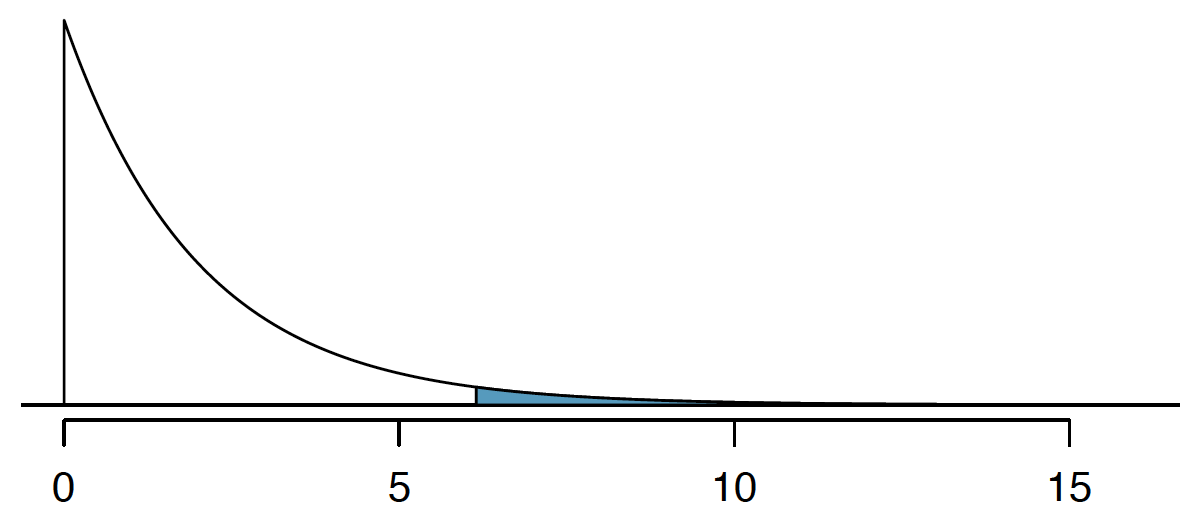
\includegraphics[height=3.5cm]{figure/pvalue.png}
%\end{center}

%\pause
%We can also compute the p-value exactly in R by typing\\
%{\tt pchisq(6.120, df=2, lower.tail=FALSE)}.  It was 0.047.

\end{frame}
%------------------------------------------------------------------------------


%------------------------------------------------------------------------------
\begin{frame}
\frametitle{Conditions/Assumptions}
Nearly identical to conditions/assumptions for $\chi^2$ tests for goodness-of-fit:
\begin{enumerate}
\pause\item \blue{Independence}:  Each case is independent of the other
\pause\item \blue{Sample size/distribution}:  We need at least 5 cases in each scenario i.e. each cell in the table
\pause\item \blue{Degrees of freedom}: (Different than before)  We need $df=(R-1)\times(C-1) \geq 2$.
\end{enumerate}

\end{frame}
%------------------------------------------------------------------------------


%------------------------------------------------------------------------------
\begin{frame}
\frametitle{Why Are They Called Degrees of Freedom?}

In the case of $\chi^2$ tests, the degrees of freedom is the number of values needed before you specify \blue{all} values in the cells of the table.

\end{frame}
%------------------------------------------------------------------------------


%------------------------------------------------------------------------------
\begin{frame}
\frametitle{Why Are They Called Degrees of Freedom? Rows}

Each row has $df=2$ because if we specify 2 values, all values in the row are specified.  

\vspace{0.5cm}

Example:
\begin{center}
  \begin{tabular}{r|ccc|c}
& \multicolumn{3}{c|}{{\tt algorithm}} & \\
       {\tt new search} & Current & Test 1 & Test 2 & Total \\ 
\hline
    No new search & X & Y &  & 7078 \\ 
    New search &  &  &  & 2922 \\ 
\hline
    Total & 5000 & 2500 & 2500 & 10000 \\ 
  \end{tabular}
\end{center}
\pause
then the missing value is $7078-X-Y$.\\ 
i.e. the \blue{wiggle room} we have is $C-1$ two cells

\end{frame}
%------------------------------------------------------------------------------


%------------------------------------------------------------------------------
\begin{frame}
\frametitle{Why Are They Called Degrees of Freedom? Columns}

Each column has $df=1$ because if we specify 1 value, all values in the column are specified.  

\vspace{0.5cm}

Example:
\begin{center}
  \begin{tabular}{r|ccc|c}
& \multicolumn{3}{c|}{{\tt algorithm}} & \\
       {\tt new search} & Current & Test 1 & Test 2 & Total \\ 
\hline
    No new search & X &  &  & 7078 \\ 
    New search &  &  &  & 2922 \\ 
\hline
    Total & 5000 & 2500 & 2500 & 10000 \\ 
  \end{tabular}
\end{center}
\pause
then the missing value is $5000-X$.\\ 
i.e. the \blue{wiggle room} we have is $R-1$ one cell

\end{frame}
%------------------------------------------------------------------------------


%------------------------------------------------------------------------------
\begin{frame}
\frametitle{Why Are They Called Degrees of Freedom? Columns}

So the overall $df$ is $(C-1)\times(R-1)$, in our case $df=2$.

\vspace{0.5cm}

\begin{center}
  \begin{tabular}{r|ccc|c}
& \multicolumn{3}{c|}{{\tt algorithm}} & \\
       {\tt new search} & Current & Test 1 & Test 2 & Total \\ 
\hline
    No new search & X & Y &  & 7078 \\ 
    New search &  &  &  & 2922 \\ 
\hline
    Total & 5000 & 2500 & 2500 & 10000 \\ 
  \end{tabular}
\end{center}
\pause
i.e. if we know these two values, we can fill the rest of the table.

\end{frame}
%------------------------------------------------------------------------------


\end{document}










